%%%%%%%%%%%%%%%%%%%%%%%%%%%%%%%%%%%%%%%%%
% Beamer Presentation
% LaTeX Template
% Version 1.0 (10/11/12)
%
% This template has been downloaded from:
% http://www.LaTeXTemplates.com
%
% License:
% CC BY-NC-SA 3.0 (http://creativecommons.org/licenses/by-nc-sa/3.0/)
%
%%%%%%%%%%%%%%%%%%%%%%%%%%%%%%%%%%%%%%%%%

%----------------------------------------------------------------------------------------
%	PACKAGES AND THEMES
%----------------------------------------------------------------------------------------

\documentclass{beamer}

\mode<presentation> {

% The Beamer class comes with a number of default slide themes
% which change the colors and layouts of slides. Below this is a list
% of all the themes, uncomment each in turn to see what they look like.

%\usetheme{default}
%\usetheme{AnnArbor}
%\usetheme{Antibes}
%\usetheme{Bergen}
%\usetheme{Berkeley}
%\usetheme{Berlin}
%\usetheme{Boadilla}
\usetheme{CambridgeUS}
%\usetheme{Copenhagen}
%\usetheme{Darmstadt}
%\usetheme{Dresden}
%\usetheme{Frankfurt}
%\usetheme{Goettingen}
%\usetheme{Hannover}
%\usetheme{Ilmenau}
%\usetheme{JuanLesPins}
%\usetheme{Luebeck}
%\usetheme{Madrid}
%\usetheme{Malmoe}
%\usetheme{Marburg}
%\usetheme{Montpellier}
%\usetheme{PaloAlto}
%\usetheme{Pittsburgh}
%\usetheme{Rochester}
%\usetheme{Singapore}
%\usetheme{Szeged}
%\usetheme{Warsaw}

% As well as themes, the Beamer class has a number of color themes
% for any slide theme. Uncomment each of these in turn to see how it
% changes the colors of your current slide theme.

%\usecolortheme{albatross}
%\usecolortheme{beaver}
%\usecolortheme{beetle}
%\usecolortheme{crane}
%\usecolortheme{dolphin}
%\usecolortheme{dove}
%\usecolortheme{fly}
%\usecolortheme{lily}
%\usecolortheme{orchid}
%\usecolortheme{rose}
%\usecolortheme{seagull}
%\usecolortheme{seahorse}
%\usecolortheme{whale}
%\usecolortheme{wolverine}

%\setbeamertemplate{footline} % To remove the footer line in all slides uncomment this line
%\setbeamertemplate{footline}[page number] % To replace the footer line in all slides with a simple slide count uncomment this line

%\setbeamertemplate{navigation symbols}{} % To remove the navigation symbols from the bottom of all slides uncomment this line
}

\usepackage{graphicx} % Allows including images
\usepackage{booktabs} % Allows the use of \toprule, \midrule and \bottomrule in tables

%----------------------------------------------------------------------------------------
%	TITLE PAGE
%----------------------------------------------------------------------------------------

\title[Examples from Legislative Studies]{Experiments on Interactive Groups, and Network Effects} % The short title appears at the bottom of every slide, the full title is only on the title page
\subtitle{Examples from Legislative Studies}

\author[]{Sayali Phadke\inst{1} \and Bruce A. Desmarais\inst{2}}
% - Give the names in the same order as the appear in the paper.
% - Use the \inst{?} command only if the authors have different
%   affiliation.

\institute[Pennsylvania State University] % (optional, but mostly needed)
{
  \inst{1}%
  PhD student\\
  Department of Statistics
  \and
  \inst{2}%
  Associate Professor\\
  Department of Political Science}

% - Use the \inst command only if there are several affiliations.
% - Keep it simple, no one is interested in your street address.

\date[JSM 2016]{Joint Statistical Meeting 2016\\~\\
\begin{tabular}{cc}
\hspace*{-.2in} \tiny \begin{minipage}{3.5in}
\small  Supported by NSF Grants: SES-1558661, SES-1619644, CISE-1320219, and DGE-1144860\\~\\
\end{minipage}
& 
\includegraphics[scale=.04]{NSF_Logo.png}
\end{tabular}
}

% - Either use conference name or its abbreviation.
% - Not really informative to the audience, more for people (including
%   yourself) who are reading the slides online

%\subject{Theoretical Computer Science}
% This is only inserted into the PDF information catalog. Can be left
% out. 

% If you have a file called "university-logo-filename.xxx", where xxx
% is a graphic format that can be processed by latex or pdflatex,
% resp., then you can add a logo as follows:

% \pgfdeclareimage[height=0.5cm]{university-logo}{university-logo-filename}
% \logo{\pgfuseimage{university-logo}}

% Delete this, if you do not want the table of contents to pop up at
% the beginning of each subsection:
%\AtBeginSubsection[]
%{
%  \begin{frame}<beamer>{Outline}
%    \tableofcontents[currentsection,currentsubsection]
%  \end{frame}
%}

\begin{document}
\begin{frame}
\titlepage % Print the title page as the first slide
\end{frame}


%%%%%%%% Slide 2: Motivation
\begin{frame}
\frametitle{Motivation: Bergan and Cole (Political Behavior, 2015)}
\begin{itemize}
\item {\LARGE Field experiment on 148 Michigan legislators}
\vspace{5mm}
\item {\LARGE Treatment: Calls from constituents}
\vspace{5mm}
\item {\LARGE Outcome: Vote on anti-bullying bill}
\vspace{5mm}
\item {\LARGE Could there have been spillover effects?}
\end{itemize}
\end{frame}


%%%%%%%% Slide 3: Overview
\begin{frame}
\frametitle{Overview} % Table of contents slide, comment this block out to remove it
\tableofcontents % Throughout your presentation, if you choose to use \section{} and \subsection{} commands, these will automatically be printed on this slide as an overview of your presentation
\end{frame}

%----------------------------------------------------------------------------------------
%	PRESENTATION SLIDES
%----------------------------------------------------------------------------------------


%%%%%%%% Slide: overview
% Section and subsections will appear in the presentation overview
% and table of contents.
\section{Motivation}

%\subsection{First Subsection}

%\begin{frame}{First Slide Title}{Optional Subtitle}
%  \begin{itemize}
%  \item {
%    My first point.
%  }
%  \item {
%    My second point.
%  }
%  \end{itemize}
%\end{frame}

%\subsection{Second Subsection}

% You can reveal the parts of a slide one at a time
% with the \pause command:
%\begin{frame}{Second Slide Title}
%  \begin{itemize}
%  \item {
%    First item.
%    \pause % The slide will pause after showing the first item
%  }
%  \item {   
%    Second item.
%  }
  % You can also specify when the content should appear
  % by using <n->:
%  \item<3-> {
%    Third item.
%  }
%  \item<4-> {
%    Fourth item.
%  }
  % or you can use the \uncover command to reveal general
  % content (not just \items):
%  \item<5-> {
%    Fifth item. \uncover<6->{Extra text in the fifth item.}
%  }
%  \end{itemize}
%\end{frame}

%\subsection{Another Subsection}

% Placing a * after \section means it will not show in the
% outline or table of contents.
%\section*{Summary}


%%%%%%%% Slide 3: Shalizi diagram
\begin{frame}
\frametitle{Motivation: Identification of causal effect}
Homophily and Contagion Are Generically Confounded in Observational Social Network Studies (Shalizi and Thomas, Sociological methods and research 2011)
\begin{figure}
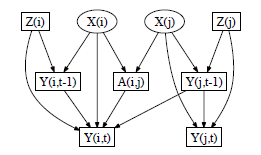
\includegraphics[width=0.7\linewidth]{Shalizi_diagram.png}
\end{figure}
\end{frame}


%%%%%%%% Slide 4: network plot
\begin{frame}
\frametitle{Motivation: Network plot}
\vspace{-5mm}
\begin{figure}
\centering
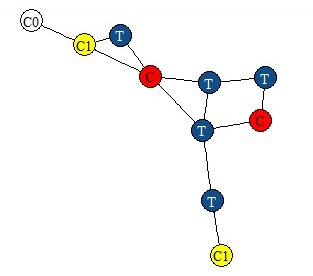
\includegraphics[width=0.5\linewidth]{Dummy_network.jpg}
\end{figure}

\vspace{-0.15cm}
\begin{block}{Stable Unit Treatment Value Assumption (SUTVA)}
Treatment status of a unit does not affect the outcome of another.
\end{block}
\end{frame}


%%%%%%%% Slide 5: research objectives
\begin{frame}
\frametitle{Research objectives}
\begin{itemize}
\item {\LARGE Model spillover of treatment effect via network structures.}
\vspace{5mm}
\item {\LARGE Examine sensitivity to specification of the model of treatment effects}
\vspace{5mm}
\item {\LARGE Evaluate models using data from field experiments on US State legislatures.}
\end{itemize}
\end{frame}


%%%%
\section{Methodology}
%%%%

%%%%%%%% Slide 6: Model intuition
\begin{frame}
\frametitle{Methodology: Intuition}
\begin{itemize}
\item {\LARGE Researcher specifies network model of effects}
\vspace{5mm}
\item {\LARGE How do we compare outcomes across groups?}
\vspace{5mm}
\item {\LARGE How do we measure effect of experiment?}
\end{itemize}
\end{frame}


%%%%%%%% Slide 7: Causal model formulation
\begin{frame}
\frametitle{Causal model (Bowers et al., Political Analysis, 2012)}
\begin{itemize}
\item {\LARGE Sharp null of no effects assumed}
\vspace{5mm}
\item {\LARGE Spillover depends on \# treated neighbors}
\vspace{5mm}
\item {\LARGE Spillover modeled as a nonlinear growth curve}
\vspace{5mm}
\item {\LARGE Separate direct and indirect effect parameters}
\end{itemize}
\end{frame}


%%%%%%%% Slide 8: Bowers method
\begin{frame}
\frametitle{Testing (Bowers et al., Political Analysis, 2012)}
\begin{itemize}
\item {\LARGE Kolmogorov-Smirnov (KS) test statistic used to compare treatment-control outcomes}
\vspace{5mm}
\item {\LARGE Compared under large number of permutations}
\vspace{5mm}
\item {\LARGE p-value is proportion of permutation statistics greater than observed statistics}
\end{itemize}
\end{frame}


%%%%%%%% Slide 9: Network
\begin{frame}
\frametitle{Salient dimensions}
\begin{itemize}
\item {\LARGE Network selection: ties through which units interact}
\vspace{5mm}
\item {\LARGE Neighborhood specification: extent of spreading of treatment}
\vspace{5mm}
\item {\LARGE Diffusion model: form taken by the spreading of treatment}
\end{itemize}
\end{frame}



%%%%
\section{Applications}
%%%%

%%%%%%%% Slide 12: NM experiment
\begin{frame}
\frametitle{Application: Butler, Nickerson et al. (2012) experiment}
\begin{itemize}
\item {\LARGE Field experiment on 70 New Mexico legislators}
\vspace{5mm}
\item {\LARGE Letters indicating constituent opinion about a spending bill}
\vspace{5mm}
\item {\LARGE Analysis concluded significant treatment effect}
\vspace{5mm}
\item {\LARGE Coppock (2014) extended analysis to model spillovers}
\end{itemize}
\end{frame}


%%%%%%%% Slide 13: Salient dimensions
\begin{frame}
\frametitle{Application: Replication of Coppock (2014)}
\vspace{-7mm}
\begin{columns}[c]

\column{.4\textwidth}
\begin{flushright}
\small {$y_{i,z} = y_{i,0} + \beta_1*z_i + \beta_2*g(\Gamma_z)$}
\end{flushright}
\centering
\begin{itemize}
\item \small {$\beta_1$ on X axis}
\vspace{2mm}
\item \small {$\beta_2$ on Y axis}
\vspace{2mm}
\item \small {Higher p-value indicates evidence for effect of experiment}
\end{itemize}

\column{.7\textwidth}
\begin{figure}
\centering
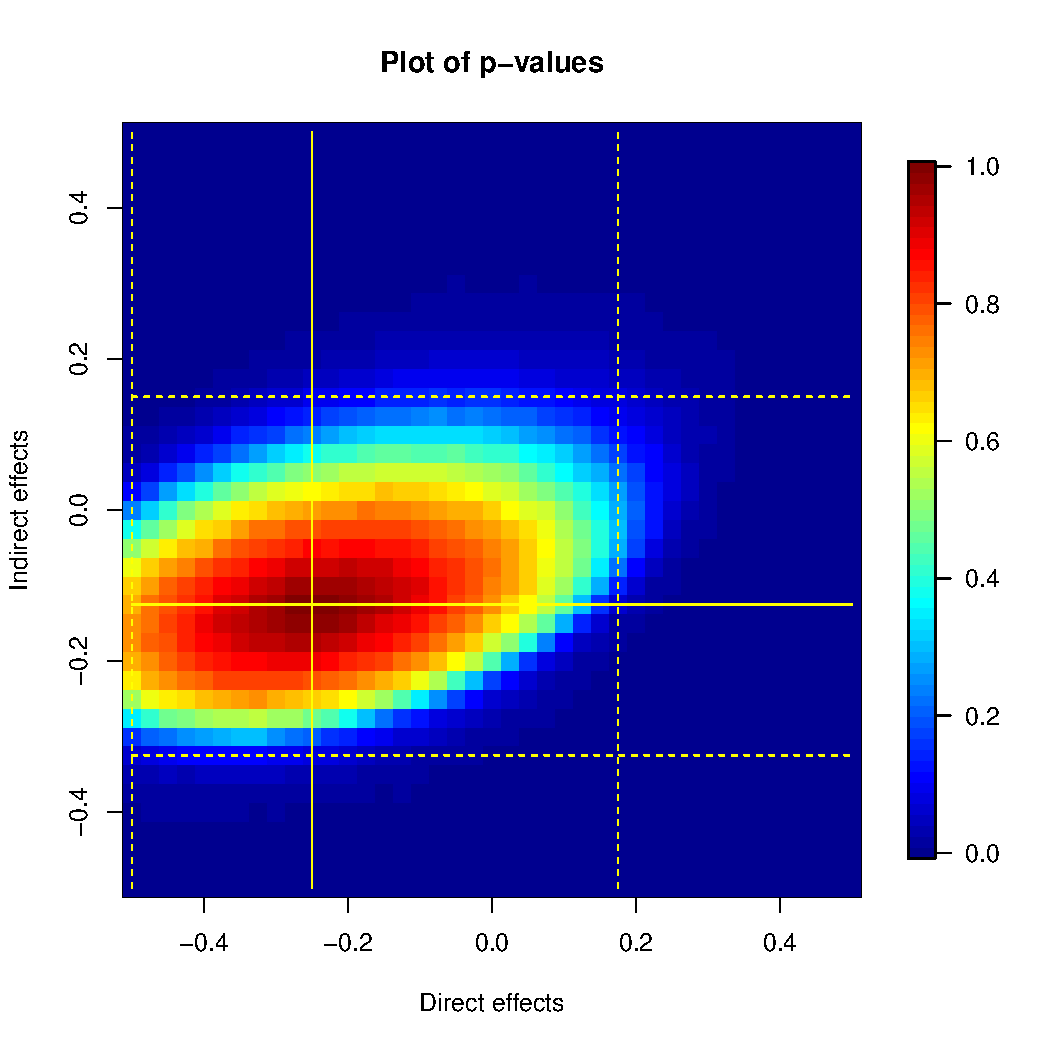
\includegraphics[scale=0.45]{pval_plot_coppock_replication.pdf}
\end{figure}

\end{columns}
\end{frame}


%%%%%%%% Slide 14: Coppock extensions 1
\begin{frame}
\frametitle{Extension: K-nearest ideological neighbors}
\vspace{-10mm}
\begin{columns}[c]

\column{.5\textwidth}
\begin{figure}
\centering
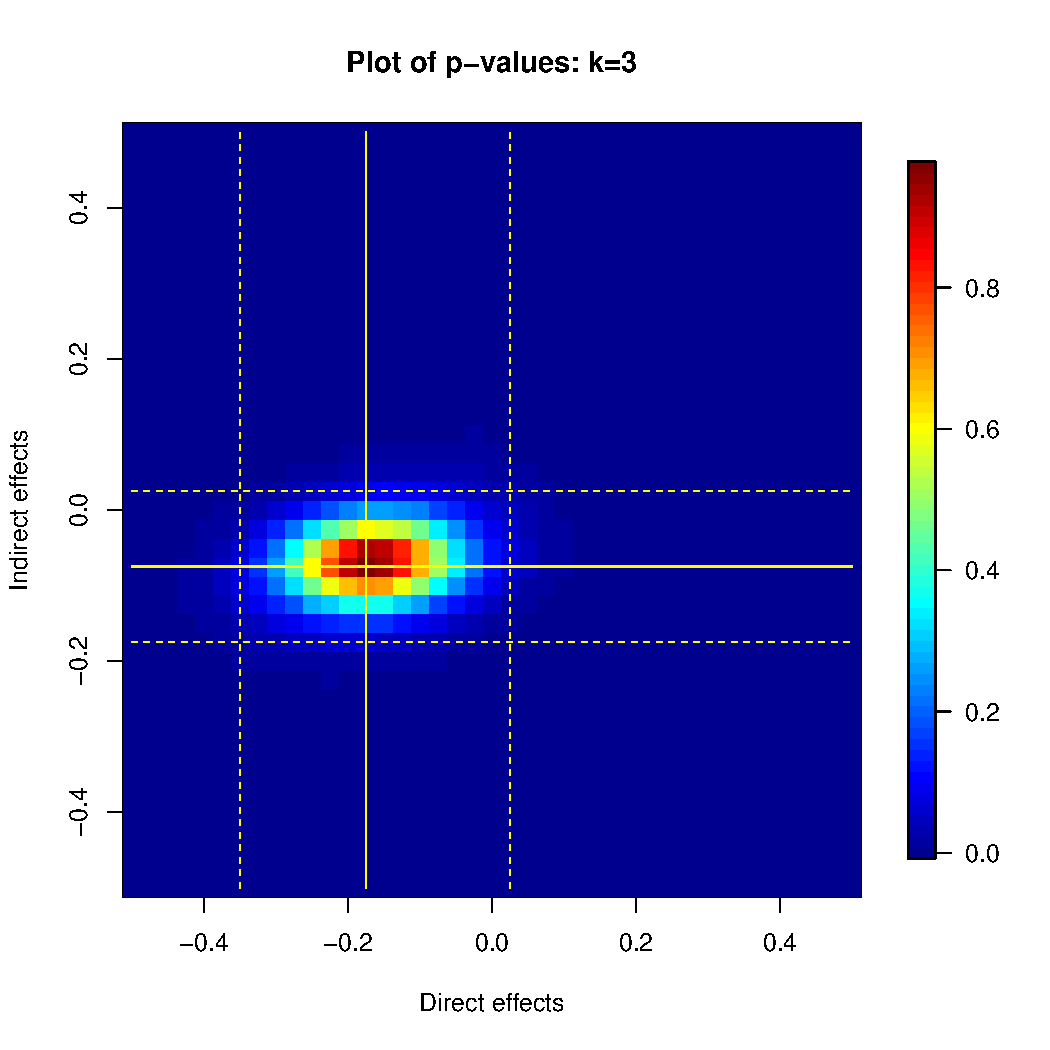
\includegraphics[trim = 11mm 0mm 9mm 0mm, clip, scale=0.39]{pval_plot_coppock_ideo_3nn.pdf}
\end{figure}

\column{.5\textwidth}
\begin{figure}
\centering
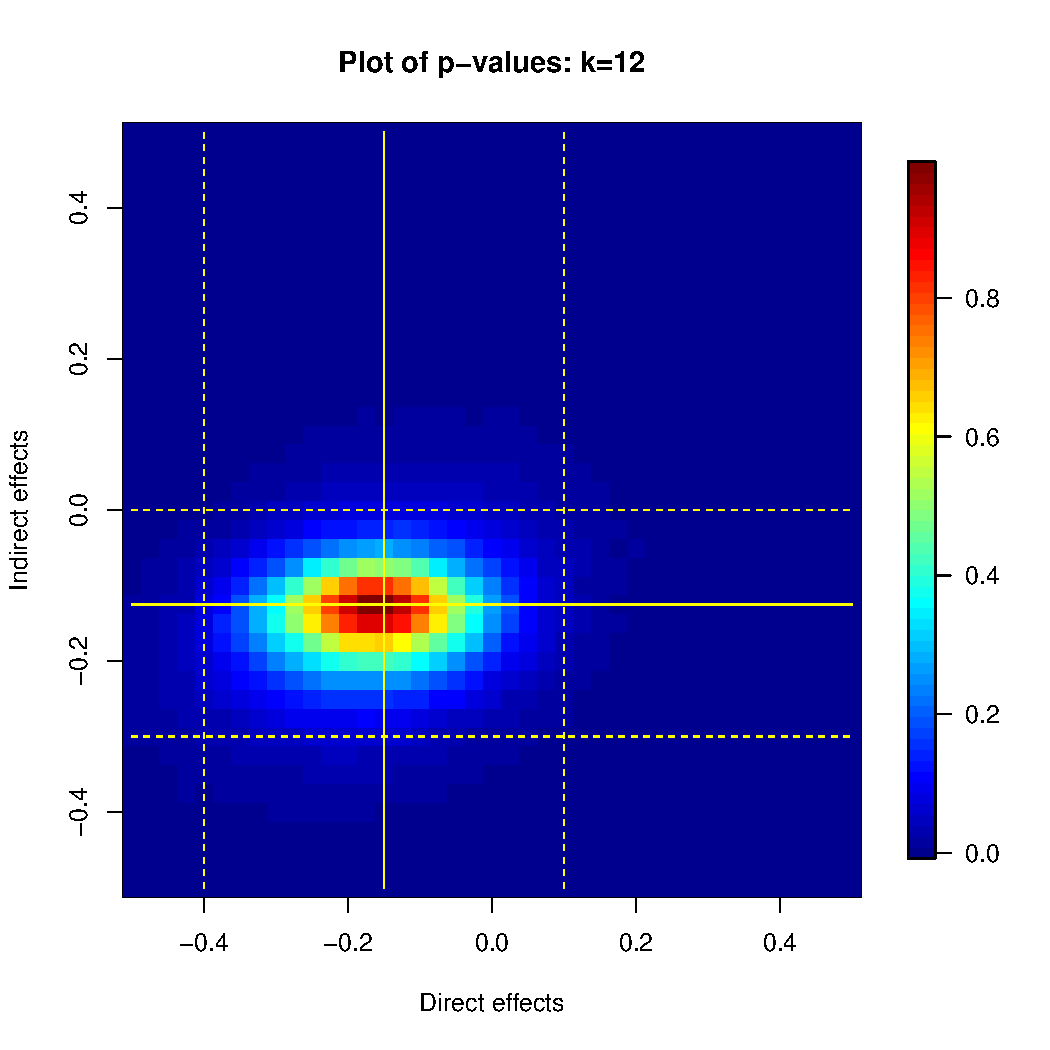
\includegraphics[trim = 11mm 0mm 9mm 0mm, clip, scale=0.39]{pval_plot_coppock_ideo_12nn.pdf}
\end{figure}

\end{columns}
\end{frame}


%%%%%%%% Slide 15: Coppock extensions 2
\begin{frame}
\frametitle{Extension: Committee network}
\vspace{-10mm}
\begin{columns}[c]

\column{.5\textwidth}
\begin{figure}
\centering
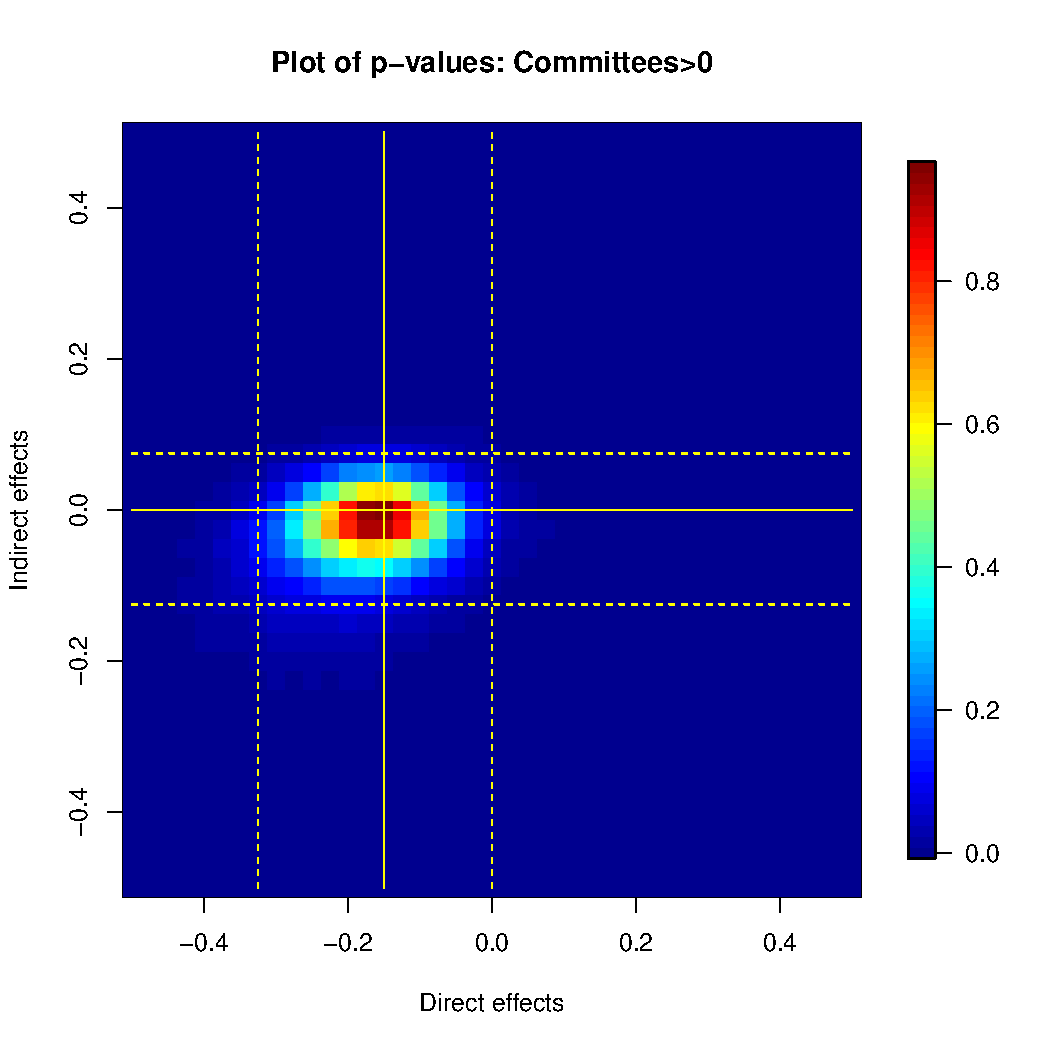
\includegraphics[trim = 11mm 0mm 9mm 0mm, clip, scale=0.39]{pval_plot_coppock_committee_1ormore.pdf}
\end{figure}

\column{.5\textwidth}
\begin{figure}
\centering
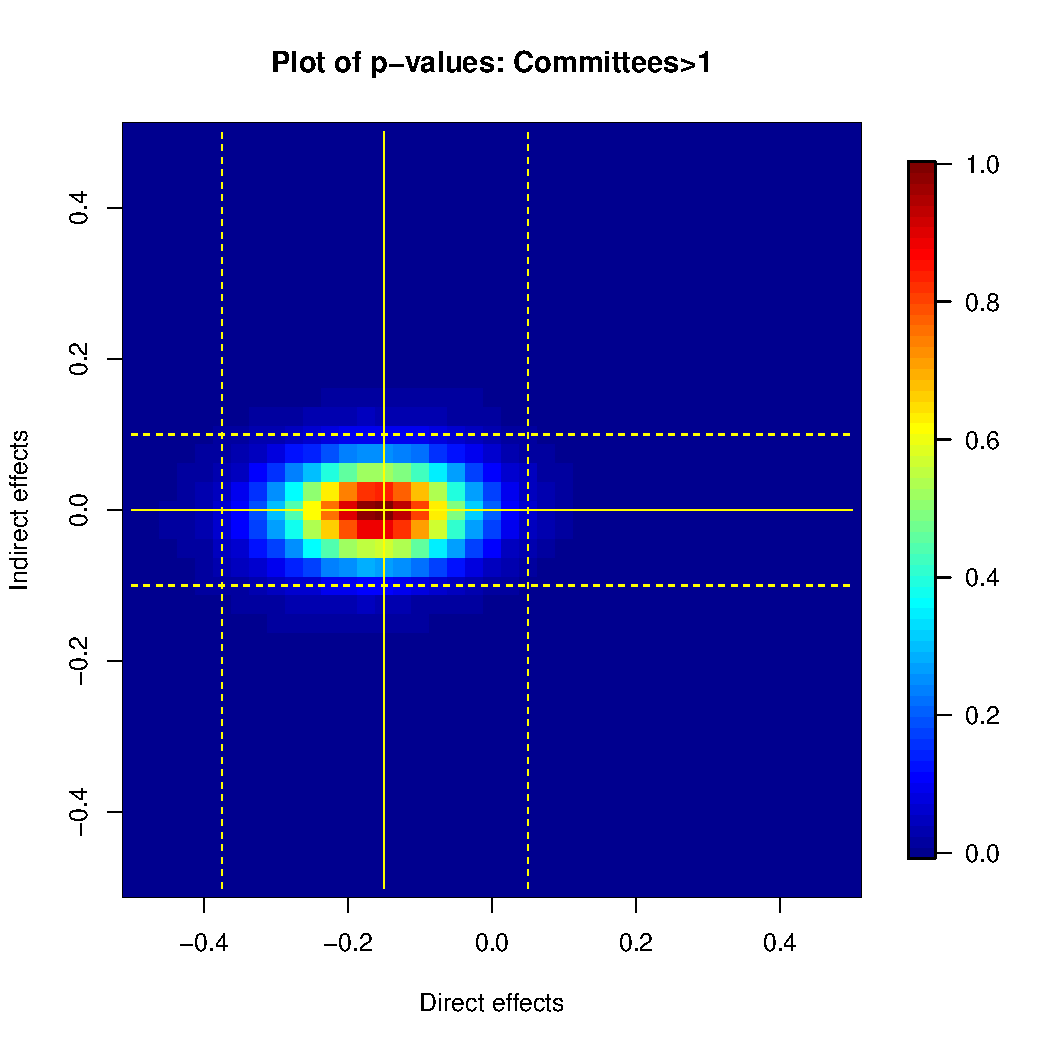
\includegraphics[trim = 11mm 0mm 9mm 0mm, clip, scale=0.39]{pval_plot_coppock_committee_2ormore.pdf}
\end{figure}

\end{columns}
\end{frame}


%%%%%%%% Slide 16: Bergan replication
\begin{frame}
\frametitle{Application: Bergan and Cole (2015)}
\vspace{-10mm}
\begin{columns}[c]

\column{.5\textwidth}
\begin{figure}
\centering
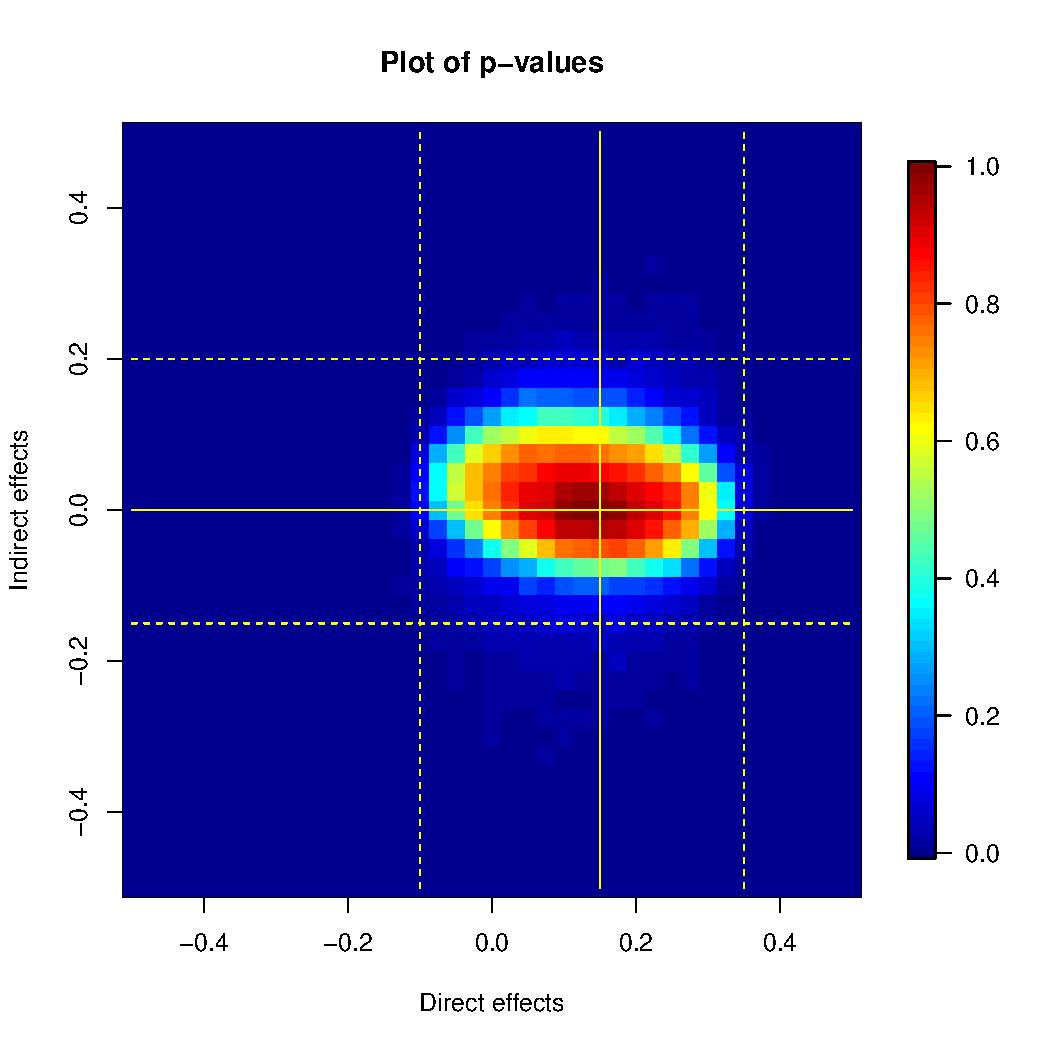
\includegraphics[trim = 11mm 0mm 9mm 0mm, clip, scale=0.39]{pval_plot_bergan_main.pdf}
\end{figure}

\column{.5\textwidth}
\begin{figure}
\centering
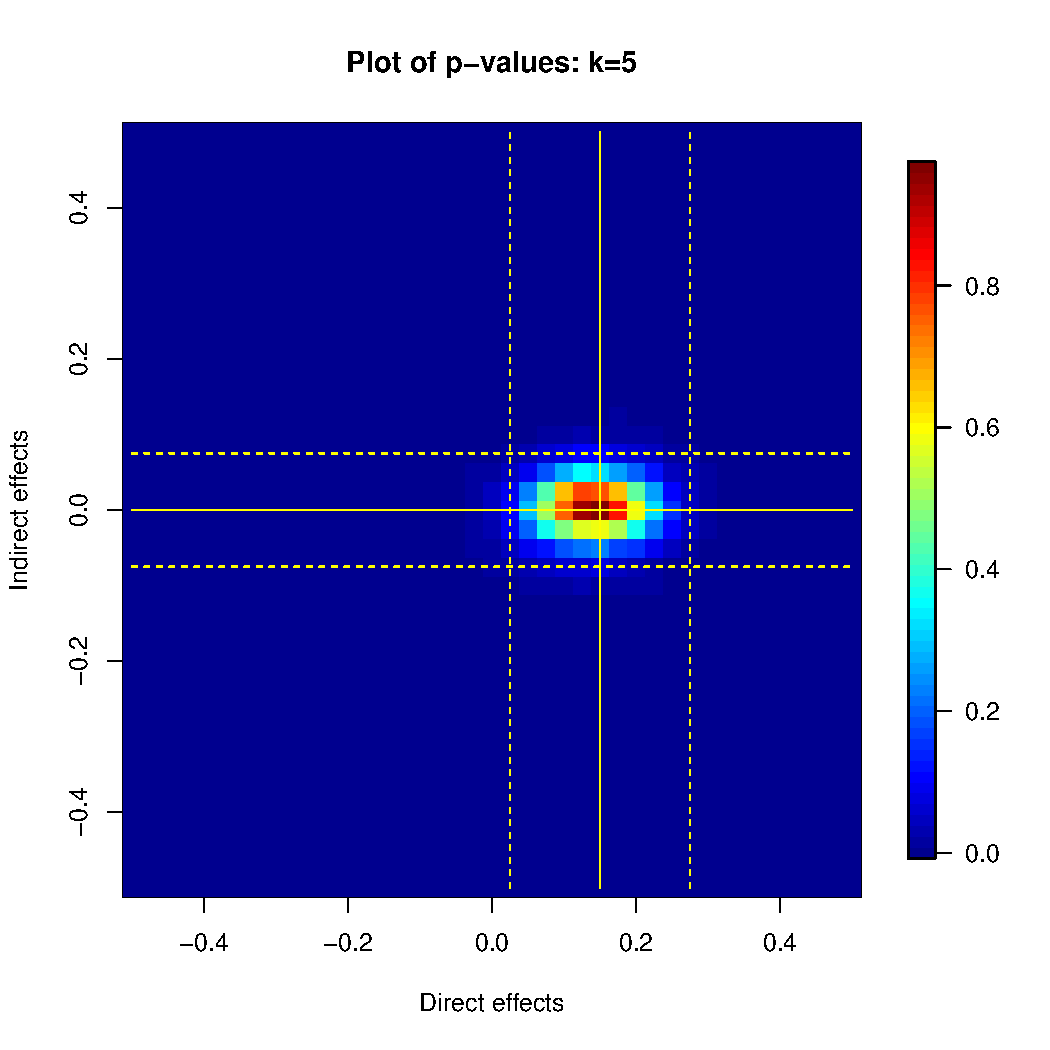
\includegraphics[trim = 11mm 0mm 9mm 0mm, clip, scale=0.39]{pval_plot_bergan_ideo_5nn.pdf}
\end{figure}

\end{columns}
\end{frame}


%%%%%%%% Slide 17: Findings
\begin{frame}
\frametitle{Replication overview}
  \begin{itemize}
 \item
   {\LARGE Treatment spreads among New Mexico legislators via ideological network}
   \vspace{5mm}
  \item
   {\LARGE Spending is a fairly partisan issue}
   \vspace{5mm}
  \item
   {\LARGE Spillover not observed among Michigan legislators}
  \end{itemize}
\end{frame}


%%%%
\section{Final remarks}
%%%%

%%%%%%%% Slide 18: Summary
\begin{frame}{Summary}
  \begin{itemize}
 \item
   {\LARGE Interference exists in experiments on interactive social groups}
   \vspace{5mm}
  \item
   {\LARGE Several dimensions important to models for interference}
   \vspace{5mm}
  \item
   {\LARGE Simulation and power analysis can assist in optimal design}
  \end{itemize}
\end{frame}


%%%%%%%% Slide 19: Next steps
\begin{frame}{Next steps}
    \begin{itemize}
	\item {\LARGE Replicate Broockman (2013) that studies legislators from multiple states}
	\vspace{5mm}
	\item {\LARGE Consider other networks}
	\vspace{5mm}
	\item {\LARGE Model a mixture of networks}
	\vspace{5mm}
	\item {\LARGE Model proportion of treated neighbors}
    \end{itemize}
\end{frame}


%%%%%%%% Slide 20: Last slide
\begin{frame}
\Huge{\centerline{Thank you}}
\vspace{5mm}
\Huge{\centerline{Questions?}}
\end{frame}


%%%%%%%% Slide 21: Appendix: networks
\begin{frame}
\frametitle{Network plots}
\begin{columns}[c]

\column{.55\textwidth}
\begin{figure}
\centering
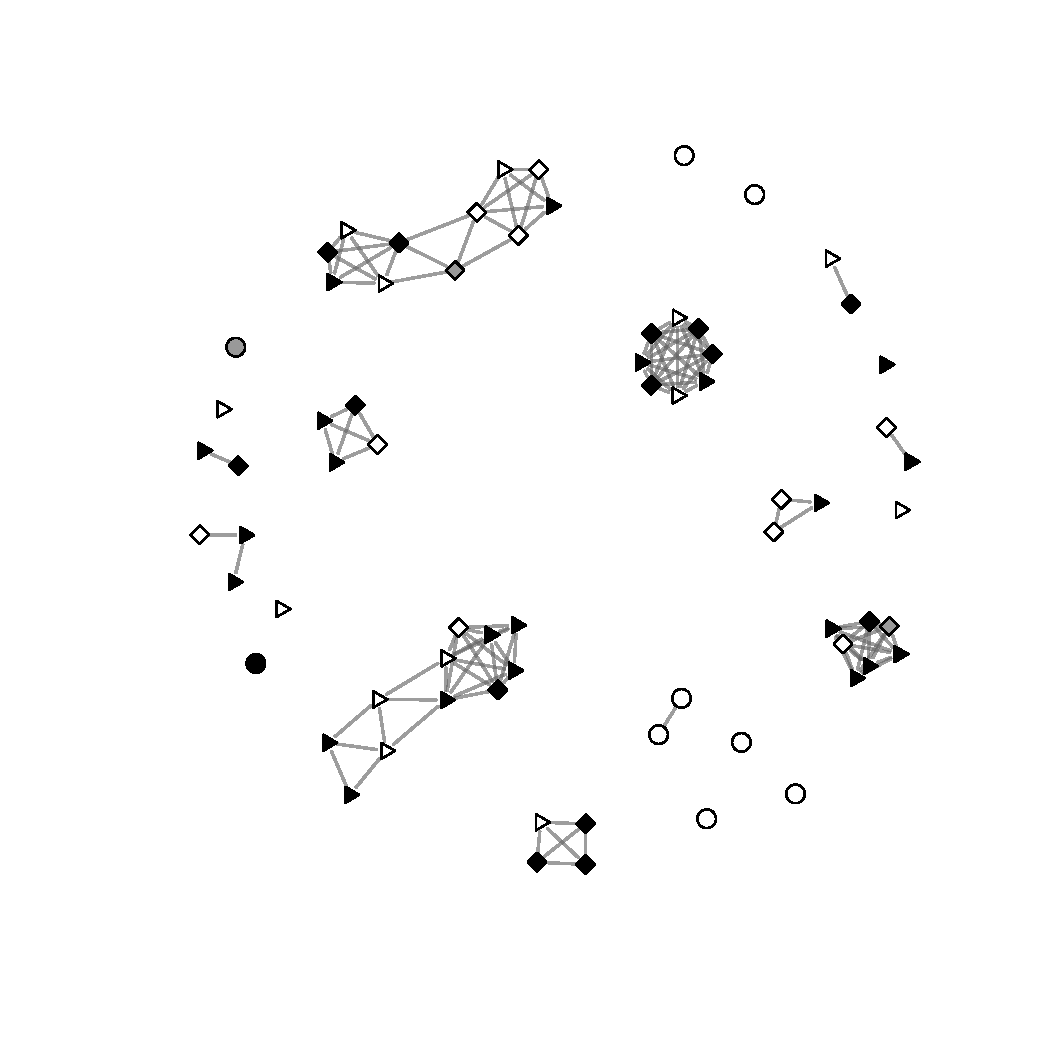
\includegraphics[scale=0.35]{Coppock_ideological_net.pdf}
\caption {Ideological network: New Mexico}
\end{figure}

\column{.55\textwidth}
\begin{figure}
\centering
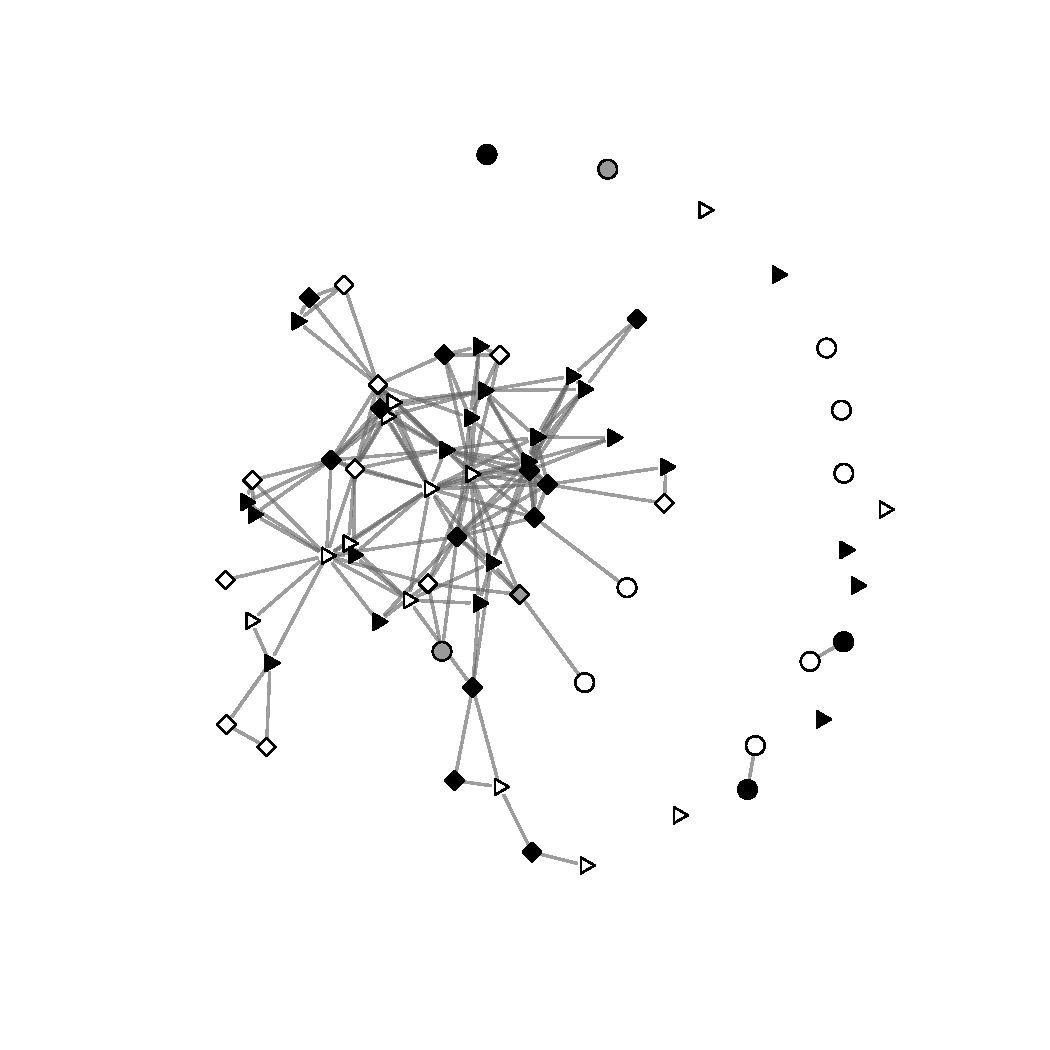
\includegraphics[scale=0.35]{Coppock_nm_committee_net.pdf}
\caption {Committee network: New Mexico}
\end{figure}

\end{columns}
\end{frame}


\end{document} 